\documentclass[tikz,border=10pt]{standalone}
\usepackage[T1]{fontenc}
\usepackage{helvet}
\renewcommand{\familydefault}{\sfdefault}
\usepackage{amsmath,amssymb}
\usepackage{tikz}
\usetikzlibrary{calc,positioning,fit,arrows.meta,shapes.geometric}

% Canonical Academic Palette
\definecolor{OxfordNavy}{HTML}{1E293B}
\definecolor{SlateSteel}{HTML}{334155}
\definecolor{MutedTeal}{HTML}{0F766E}
\definecolor{TealL0}{HTML}{F0FDFA}
\definecolor{Burgundy}{HTML}{991B1B}
\definecolor{BurgundyL0}{HTML}{FEF2F2}
\definecolor{WarmOchre}{HTML}{92400E}
\definecolor{OchreL0}{HTML}{FFFBEB}
\definecolor{ForestSage}{HTML}{166534}
\definecolor{SageL0}{HTML}{F0FDF4}
\definecolor{CoolParchment}{HTML}{F8FAFC}
\definecolor{SlateRim}{HTML}{CBD5E1}
\definecolor{GoldPin}{HTML}{D97706}
\definecolor{DarkSlate}{HTML}{0F172A}

\begin{document}
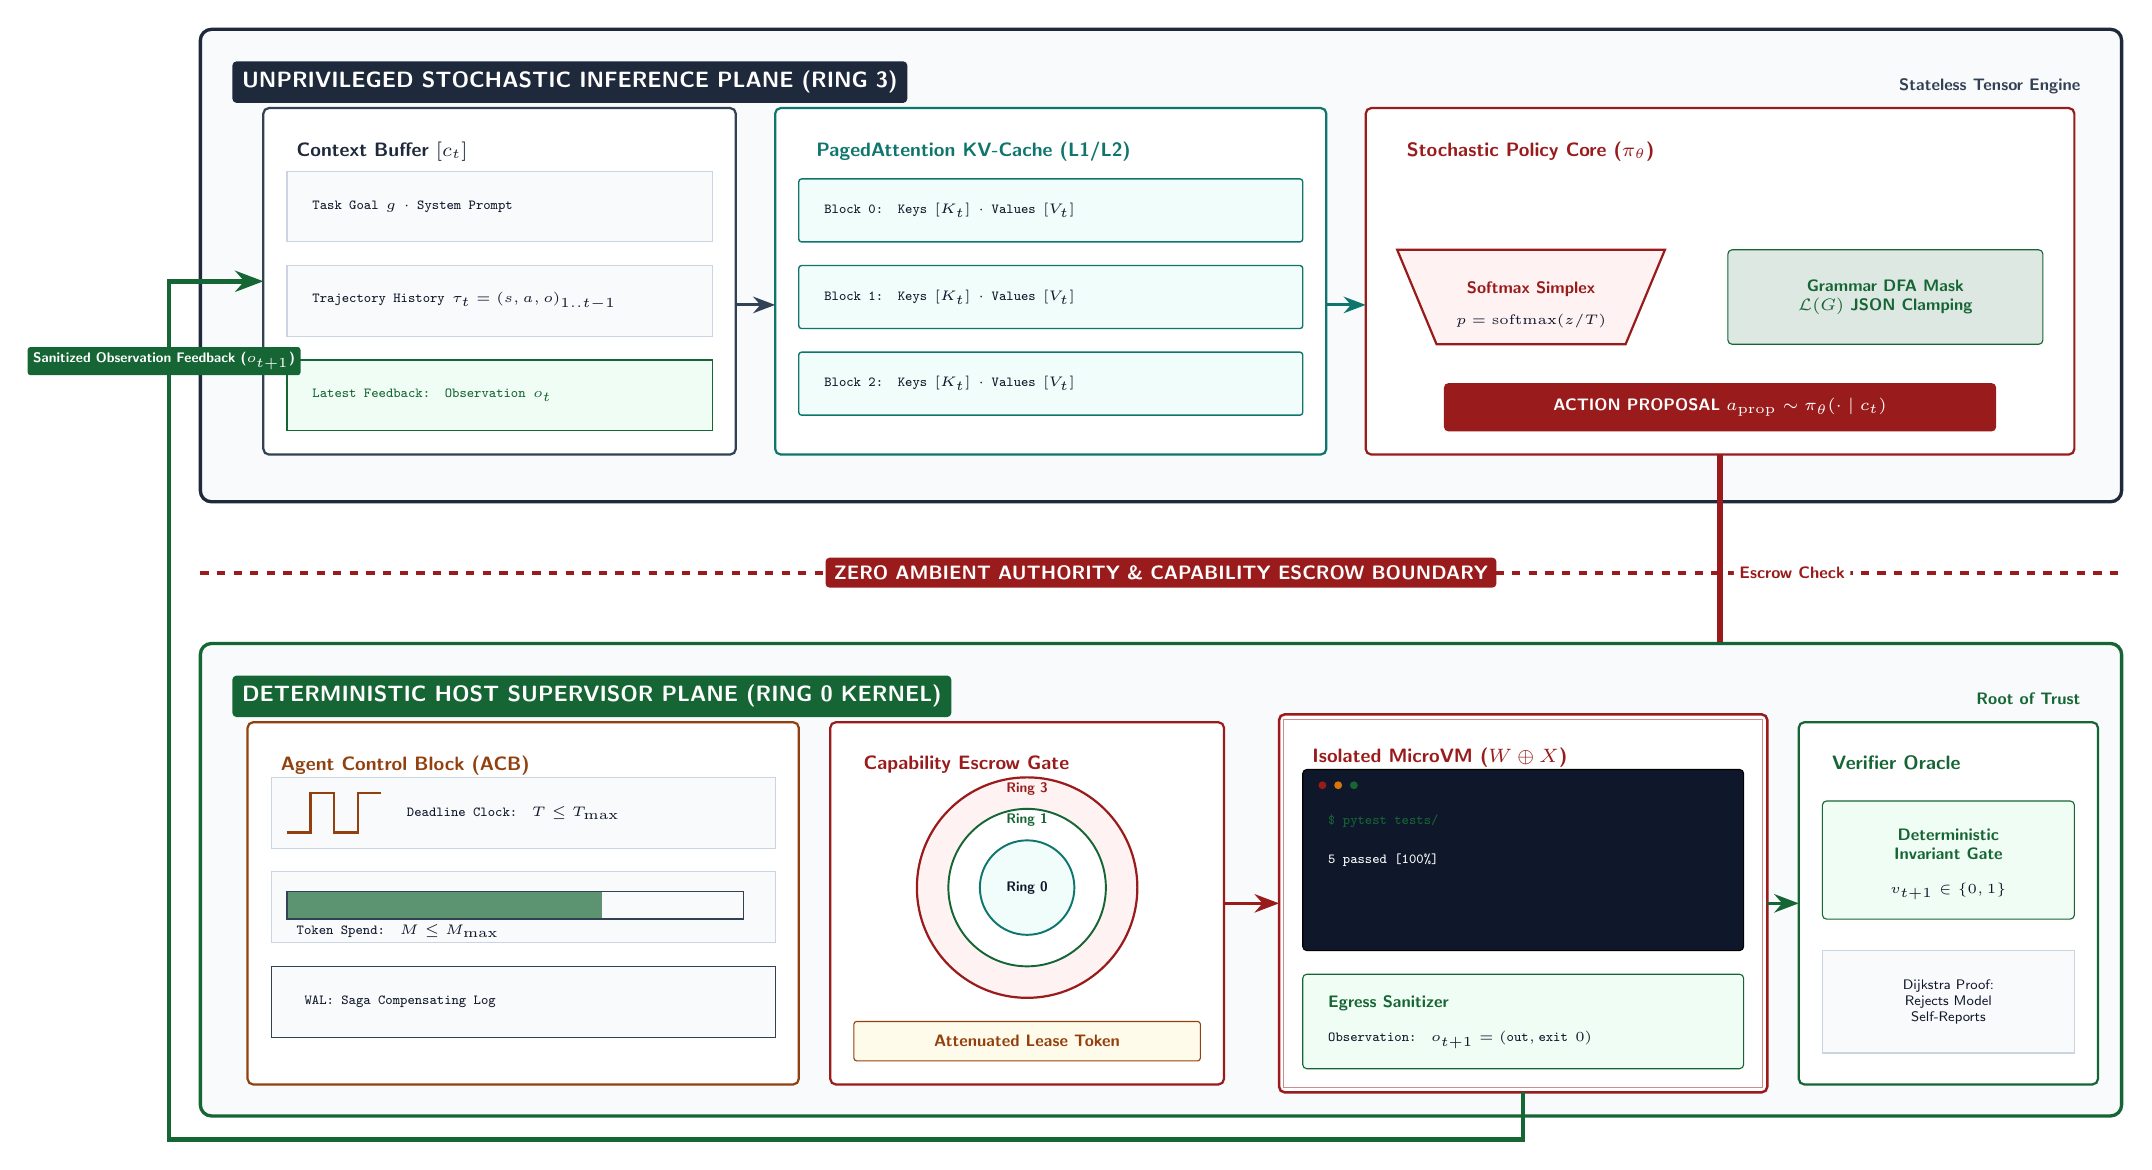
\begin{tikzpicture}[
  font=\sffamily,
  scale=1.0,
  >=Stealth
]

% -------------------------------------------------------------
% TOP PLANE: UNPRIVILEGED STOCHASTIC INFERENCE (RING 3)
% -------------------------------------------------------------
\draw[fill=CoolParchment, draw=OxfordNavy, line width=1.2pt, rounded corners=4pt]
  (0, 8.2) rectangle (24.4, 14.2);

\node[anchor=north west, fill=OxfordNavy, text=white, font=\fontsize{8.5}{10}\selectfont\bfseries, rounded corners=1.5pt, inner sep=3.5pt]
  at (0.4, 13.8) {UNPRIVILEGED STOCHASTIC INFERENCE PLANE (RING 3)};
\node[anchor=north east, text=SlateSteel, font=\fontsize{6.5}{8}\selectfont\bfseries]
  at (24.0, 13.7) {Stateless Tensor Engine};

% Context Buffer
\begin{scope}[shift={(0.8, 8.8)}]
  \draw[fill=white, draw=SlateSteel, line width=0.8pt, rounded corners=2pt] (0, 0) rectangle (6.0, 4.4);
  \node[anchor=north west, text=OxfordNavy, font=\fontsize{7.5}{9}\selectfont\bfseries] at (0.3, 4.1) {Context Buffer $[c_t]$};

  \draw[fill=CoolParchment, draw=SlateRim] (0.3, 2.7) rectangle (5.7, 3.6);
  \node[anchor=west, text=DarkSlate, font=\fontsize{5.5}{6.5}\selectfont\ttfamily] at (0.5, 3.15) {Task Goal $g$ $\cdot$ System Prompt};

  \draw[fill=CoolParchment, draw=SlateRim] (0.3, 1.5) rectangle (5.7, 2.4);
  \node[anchor=west, text=DarkSlate, font=\fontsize{5.5}{6.5}\selectfont\ttfamily] at (0.5, 1.95) {Trajectory History $\tau_t = (s, a, o)_{1..t-1}$};

  \draw[fill=SageL0, draw=ForestSage] (0.3, 0.3) rectangle (5.7, 1.2);
  \node[anchor=west, text=ForestSage, font=\fontsize{5.5}{6.5}\selectfont\ttfamily\bfseries] at (0.5, 0.75) {Latest Feedback: Observation $o_t$};
\end{scope}

% PagedAttention KV-Cache
\begin{scope}[shift={(7.3, 8.8)}]
  \draw[fill=white, draw=MutedTeal, line width=0.8pt, rounded corners=2pt] (0, 0) rectangle (7.0, 4.4);
  \node[anchor=north west, text=MutedTeal, font=\fontsize{7.5}{9}\selectfont\bfseries] at (0.4, 4.1) {PagedAttention KV-Cache (L1/L2)};

  \foreach \b in {0, 1, 2} {
    \draw[fill=TealL0, draw=MutedTeal, line width=0.5pt, rounded corners=1pt] (0.3, 2.7 - \b*1.1) rectangle (6.7, 3.5 - \b*1.1);
    \node[anchor=west, text=DarkSlate, font=\fontsize{5.5}{6.5}\selectfont\ttfamily] at (0.5, 3.1 - \b*1.1) {Block \b: Keys $[K_t]$ $\cdot$ Values $[V_t]$};
  }
\end{scope}

% Stochastic Policy Core
\begin{scope}[shift={(14.8, 8.8)}]
  \draw[fill=white, draw=Burgundy, line width=0.8pt, rounded corners=2pt] (0, 0) rectangle (9.0, 4.4);
  \node[anchor=north west, text=Burgundy, font=\fontsize{7.5}{9}\selectfont\bfseries] at (0.4, 4.1) {Stochastic Policy Core ($\pi_\theta$)};

  % Trapezoidal Sampler
  \draw[fill=BurgundyL0, draw=Burgundy, line width=0.8pt] 
    (0.4, 2.6) -- (3.8, 2.6) -- (3.3, 1.4) -- (0.9, 1.4) -- cycle;
  \node[text=Burgundy, font=\fontsize{6.2}{7.5}\selectfont\bfseries] at (2.1, 2.1) {Softmax Simplex};
  \node[text=DarkSlate, font=\fontsize{5.2}{6}\selectfont] at (2.1, 1.7) {$p = \mathrm{softmax}(z/T)$};

  % DFA Grammar
  \begin{scope}[shift={(4.6, 1.4)}]
    \draw[fill=ForestSage!15, draw=ForestSage, rounded corners=1.5pt] (0, 0) rectangle (4.0, 1.2);
    \node[text=ForestSage, font=\fontsize{6.0}{7}\selectfont\bfseries, align=center] at (2.0, 0.6) {Grammar DFA Mask\\$\mathcal{L}(G)$ JSON Clamping};
  \end{scope}

  % Output proposal
  \draw[fill=Burgundy, draw=Burgundy, rounded corners=1.5pt] (1.0, 0.3) rectangle (8.0, 0.9);
  \node[text=white, font=\fontsize{6.2}{7.5}\selectfont\bfseries] at (4.5, 0.6) {ACTION PROPOSAL $a_{\mathrm{prop}} \sim \pi_\theta(\cdot \mid c_t)$};
\end{scope}

% Signal connections in top plane
\draw[->, draw=SlateSteel, line width=1.1pt] (6.8, 10.7) -- (7.3, 10.7);
\draw[->, draw=MutedTeal, line width=1.1pt] (14.3, 10.7) -- (14.8, 10.7);


% -------------------------------------------------------------
% HORIZONTAL FIREWALL: ZERO AMBIENT AUTHORITY BOUNDARY
% -------------------------------------------------------------
\draw[draw=Burgundy, line width=1.4pt, dashed] (0, 7.3) -- (24.4, 7.3);
\node[fill=Burgundy, text=white, font=\fontsize{7.0}{8.5}\selectfont\bfseries, rounded corners=1.5pt, inner sep=3pt]
  at (12.2, 7.3) {ZERO AMBIENT AUTHORITY \& CAPABILITY ESCROW BOUNDARY};

% Proposal crossing the boundary (clean white background mask on Escrow Check label)
\draw[->, draw=Burgundy, line width=2.0pt] (19.3, 8.8) -- (19.3, 5.8)
  node[midway, fill=white, inner sep=2pt, rounded corners=1pt, right=4pt, font=\fontsize{6.0}{7}\selectfont\bfseries, text=Burgundy] {Escrow Check};


% -------------------------------------------------------------
% BOTTOM PLANE: DETERMINISTIC HOST SUPERVISOR & ACTUATION
% -------------------------------------------------------------
\draw[fill=CoolParchment, draw=ForestSage, line width=1.2pt, rounded corners=4pt]
  (0, 0.4) rectangle (24.4, 6.4);

\node[anchor=north west, fill=ForestSage, text=white, font=\fontsize{8.5}{10}\selectfont\bfseries, rounded corners=1.5pt, inner sep=3.5pt]
  at (0.4, 6.0) {DETERMINISTIC HOST SUPERVISOR PLANE (RING 0 KERNEL)};
\node[anchor=north east, text=ForestSage, font=\fontsize{6.5}{8}\selectfont\bfseries]
  at (24.0, 5.9) {Root of Trust};

% Host Supervisor Control Box (ACB)
\begin{scope}[shift={(0.6, 0.8)}]
  \draw[fill=white, draw=WarmOchre, line width=0.8pt, rounded corners=2pt] (0, 0) rectangle (7.0, 4.6);
  \node[anchor=north west, text=WarmOchre, font=\fontsize{7.5}{9}\selectfont\bfseries] at (0.3, 4.3) {Agent Control Block (ACB)};

  % Clock
  \begin{scope}[shift={(0.3, 3.0)}]
    \draw[fill=CoolParchment, draw=SlateRim] (0, 0) rectangle (6.4, 0.9);
    \draw[draw=WarmOchre, line width=0.9pt]
      (0.2, 0.2) -- (0.5, 0.2) -- (0.5, 0.7) -- (0.8, 0.7) -- (0.8, 0.2) -- (1.1, 0.2) -- (1.1, 0.7) -- (1.4, 0.7);
    \node[anchor=west, text=DarkSlate, font=\fontsize{5.5}{6.5}\selectfont\ttfamily] at (1.6, 0.45) {Deadline Clock: $T \le T_{\max}$};
  \end{scope}

  % Fuel
  \begin{scope}[shift={(0.3, 1.8)}]
    \draw[fill=CoolParchment, draw=SlateRim] (0, 0) rectangle (6.4, 0.9);
    \fill[ForestSage!70] (0.2, 0.3) rectangle (4.2, 0.65);
    \draw[draw=SlateSteel, line width=0.5pt] (0.2, 0.3) rectangle (6.0, 0.65);
    \node[anchor=west, text=DarkSlate, font=\fontsize{5.5}{6.5}\selectfont\ttfamily] at (0.2, 0.15) {Token Spend: $M \le M_{\max}$};
  \end{scope}

  % WAL
  \begin{scope}[shift={(0.3, 0.6)}]
    \draw[fill=CoolParchment, draw=SlateSteel] (0, 0) rectangle (6.4, 0.9);
    \node[anchor=west, text=DarkSlate, font=\fontsize{5.5}{6.5}\selectfont\ttfamily\bfseries] at (0.3, 0.45) {WAL: Saga Compensating Log};
  \end{scope}
\end{scope}

% Capability Escrow Gate
\begin{scope}[shift={(8.0, 0.8)}]
  \draw[fill=white, draw=Burgundy, line width=0.8pt, rounded corners=2pt] (0, 0) rectangle (5.0, 4.6);
  \node[anchor=north west, text=Burgundy, font=\fontsize{7.5}{9}\selectfont\bfseries] at (0.3, 4.3) {Capability Escrow Gate};

  \begin{scope}[shift={(2.5, 2.5)}]
    \draw[draw=Burgundy, fill=BurgundyL0, line width=0.8pt] (0, 0) circle (1.4);
    \node[anchor=south, font=\fontsize{5.0}{6}\selectfont\bfseries, text=Burgundy] at (0, 1.05) {Ring 3};

    \draw[draw=ForestSage, fill=white, line width=0.7pt] (0, 0) circle (1.0);
    \node[anchor=south, font=\fontsize{5.0}{6}\selectfont\bfseries, text=ForestSage] at (0, 0.65) {Ring 1};

    \draw[draw=MutedTeal, fill=TealL0, line width=0.7pt] (0, 0) circle (0.6);
    \node[font=\fontsize{5.5}{6.5}\selectfont\bfseries, text=DarkSlate] at (0, 0) {Ring 0};
  \end{scope}

  \draw[fill=OchreL0, draw=WarmOchre, rounded corners=1pt] (0.3, 0.3) rectangle (4.7, 0.8);
  \node[font=\fontsize{6.0}{7}\selectfont\bfseries, text=WarmOchre] at (2.5, 0.55) {Attenuated Lease Token};
\end{scope}

\draw[->, draw=Burgundy, line width=1.3pt] (13.0, 3.1) -- (13.7, 3.1);

% Isolated MicroVM
\begin{scope}[shift={(13.7, 0.7)}]
  \draw[fill=white, draw=Burgundy, line width=0.9pt, rounded corners=2pt] (0, 0) rectangle (6.2, 4.8);
  \draw[draw=Burgundy!50, line width=0.4pt] (0.06, 0.06) rectangle (6.14, 4.74);
  \node[anchor=north west, text=Burgundy, font=\fontsize{7.2}{8.5}\selectfont\bfseries] at (0.3, 4.5) {Isolated MicroVM ($W \oplus X$)};

  % Terminal
  \begin{scope}[shift={(0.3, 1.8)}]
    \draw[fill=DarkSlate, draw=black, rounded corners=1.5pt] (0, 0) rectangle (5.6, 2.3);
    \fill[Burgundy] (0.25, 2.1) circle (0.05);
    \fill[GoldPin] (0.45, 2.1) circle (0.05);
    \fill[ForestSage] (0.65, 2.1) circle (0.05);
    \node[anchor=north west, font=\fontsize{4.6}{5.5}\selectfont\ttfamily, text=ForestSage] at (0.2, 1.85) {\$ pytest tests/};
    \node[anchor=north west, font=\fontsize{4.4}{5.5}\selectfont\ttfamily, text=white!90] at (0.2, 1.35) {5 passed [100\%]};
  \end{scope}

  % Egress Sanitizer
  \begin{scope}[shift={(0.3, 0.3)}]
    \draw[fill=SageL0, draw=ForestSage, rounded corners=1.5pt] (0, 0) rectangle (5.6, 1.2);
    \node[anchor=north west, text=ForestSage, font=\fontsize{6.0}{7}\selectfont\bfseries] at (0.2, 1.05) {Egress Sanitizer};
    \node[anchor=north west, text=DarkSlate, font=\fontsize{4.6}{5.5}\selectfont\ttfamily] at (0.2, 0.6) {Observation: $o_{t+1} = (\text{out}, \text{exit } 0)$};
  \end{scope}
\end{scope}

% Verifier Oracle
\begin{scope}[shift={(20.3, 0.8)}]
  \draw[fill=white, draw=ForestSage, line width=0.8pt, rounded corners=2pt] (0, 0) rectangle (3.8, 4.6);
  \node[anchor=north west, text=ForestSage, font=\fontsize{7.0}{8.5}\selectfont\bfseries] at (0.3, 4.3) {Verifier Oracle};

  \draw[fill=SageL0, draw=ForestSage, rounded corners=1.5pt] (0.3, 2.1) rectangle (3.5, 3.6);
  \node[font=\fontsize{5.8}{7}\selectfont\bfseries, text=ForestSage, align=center] at (1.9, 3.05) {Deterministic\\Invariant Gate};
  \node[font=\fontsize{5.0}{6}\selectfont\ttfamily, text=DarkSlate] at (1.9, 2.45) {$v_{t+1} \in \{0, 1\}$};

  \draw[fill=CoolParchment, draw=SlateRim] (0.3, 0.4) rectangle (3.5, 1.7);
  \node[font=\fontsize{4.8}{5.8}\selectfont, text=DarkSlate, align=center] at (1.9, 1.05) {Dijkstra Proof:\\Rejects Model\\Self-Reports};
\end{scope}

\draw[->, draw=ForestSage, line width=1.3pt] (19.9, 3.1) -- (20.3, 3.1);

% Closed Feedback Loop back to Context Buffer in Ring 3
\draw[->, draw=ForestSage, line width=1.6pt]
  (16.8, 0.7) -- (16.8, 0.1) -- (-0.4, 0.1) -- (-0.4, 11.0) -- (0.8, 11.0);

\node[anchor=south west, fill=ForestSage, text=white, font=\fontsize{5.5}{6.5}\selectfont\bfseries, rounded corners=1pt, inner sep=2pt]
  at (-2.2, 9.8) {Sanitized Observation Feedback ($o_{t+1}$)};

\end{tikzpicture}
\end{document}
